% ============================================================
%  Capítulo 7 — Diseño de la Solución
% ============================================================

\section{Diseño de la Solución}

Este capítulo describe las decisiones de diseño adoptadas para materializar los
requisitos funcionales y no funcionales de OmniLitter en una arquitectura concreta.
Se abordan, en orden de abstracción descendente, la arquitectura general del sistema,
el diseño de la base de datos, el contrato de la API REST, la estructura de componentes
del portal web y de la aplicación móvil, y el mecanismo de sincronización \textit{offline}.

% ------------------------------------------------------------
\subsection{Visión General de la Arquitectura}
% ------------------------------------------------------------

OmniLitter sigue una arquitectura de \textbf{tres capas} clásica adaptada a un
contexto multiplataforma con requisito de operación sin conexión:

\begin{enumerate}
  \item \textbf{Capa de presentación.} Comprende dos clientes independientes: el portal web,
    orientado a la consulta y gestión de datos por parte de investigadores y administradores, y
    la aplicación móvil, orientada a la captura de observaciones en campo.
  \item \textbf{Capa de lógica de negocio.} Una API REST centralizada implementada en
    Node.js + Express actúa como único punto de acceso a los datos, aplica las reglas de
    negocio y gestiona la autenticación mediante \textit{tokens} JWT.
  \item \textbf{Capa de persistencia.} PostgreSQL almacena el estado canónico del sistema.
    Adicionalmente, la aplicación móvil mantiene una base de datos local con WatermelonDB
    (capa sobre SQLite) que permite operar sin conexión y sincronizarse en diferido.
\end{enumerate}

La figura~\ref{fig:arquitectura} muestra un diagrama de la arquitectura del sistema.

\begin{figure}[H]
  \centering
  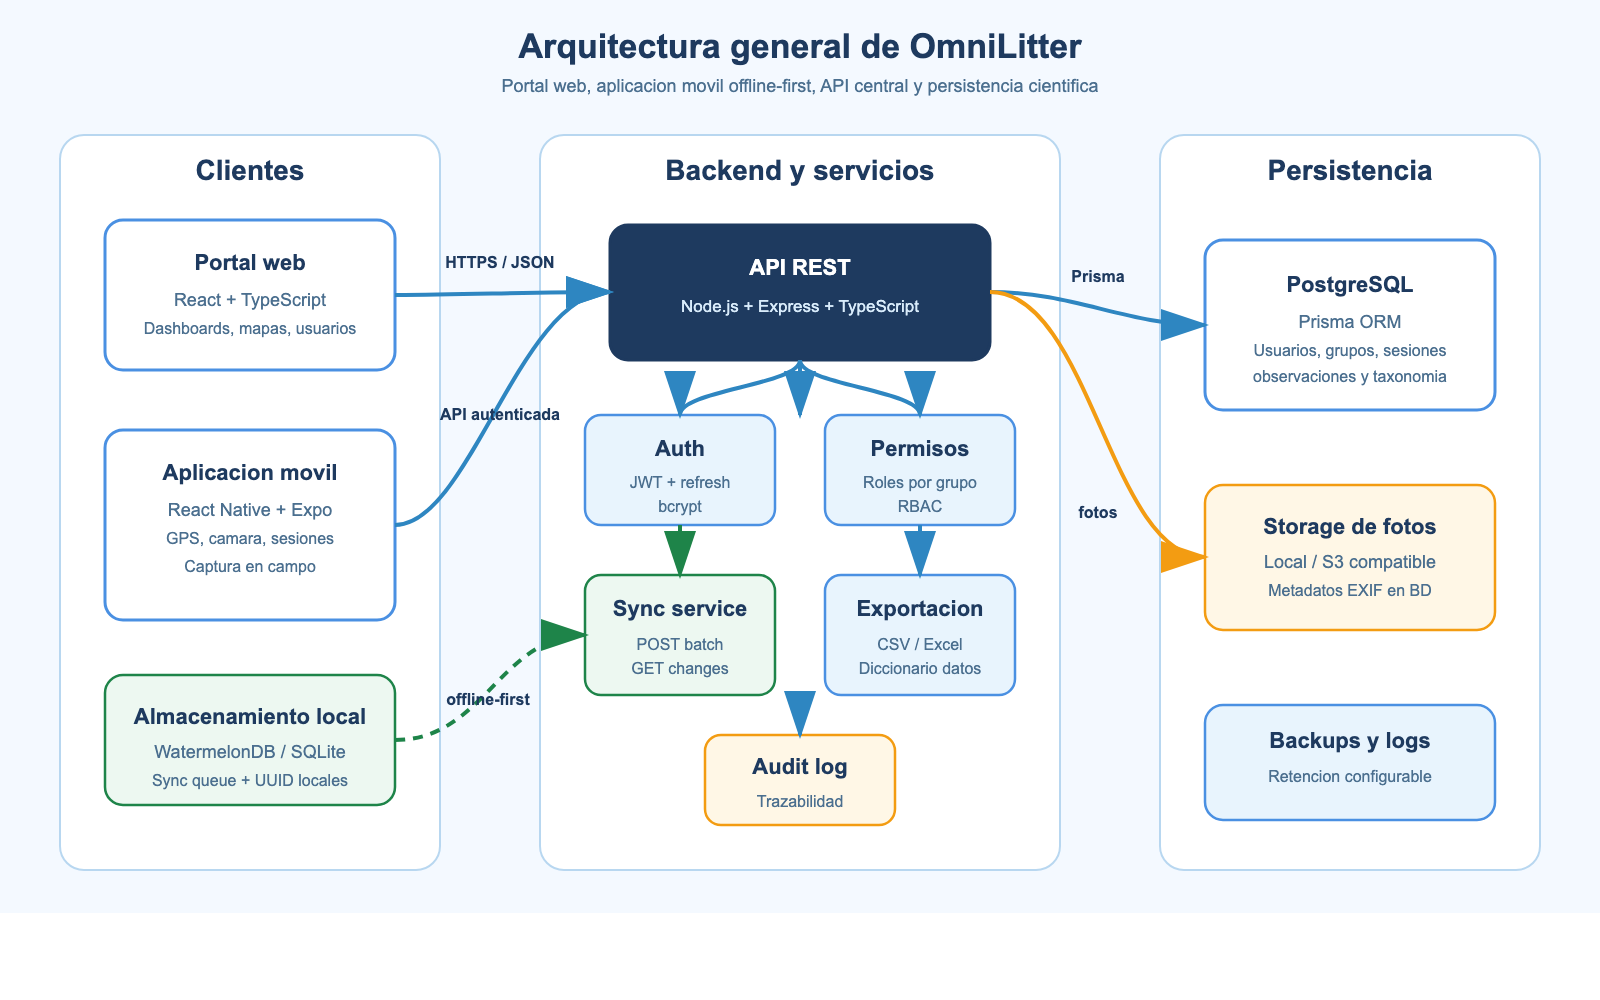
\includegraphics[width=0.8\textwidth]{figures/arquitectura.png}
  \caption{Arquitectura general propuesta para OmniLitter.}
  \label{fig:arquitectura}
\end{figure}


\subsubsection{Justificación de las decisiones arquitectónicas principales}

\textbf{API REST como único punto de acceso.}
Centralizar la lógica de negocio en la API evita duplicidades entre los dos clientes y
facilita la incorporación de nuevos consumidores en el futuro (p.ej., exportaciones
automatizadas por \textit{scripts} externos o integraciones con repositorios científicos).

\textbf{Separación entre portal web y aplicación móvil.}
Aunque comparten la misma API, los dos clientes tienen requisitos de experiencia de usuario
muy distintos: el portal prioriza la visualización analítica y la gestión, mientras que la
app móvil prioriza la captura rápida en condiciones de campo adversas (luz solar, guantes,
sin conexión). Mantenerlos como proyectos independientes permite evolucionar cada uno a su
propio ritmo.

\textbf{Base de datos local en el móvil.}
El trabajo de campo se realiza habitualmente en zonas costeras, ribereñas o forestales
con cobertura de red intermitente o nula. La decisión de embeber una base de datos local en
el dispositivo es, por tanto, un requisito no negociable para la viabilidad del producto.

% ------------------------------------------------------------
\subsection{Diseño de la Base de Datos}
% ------------------------------------------------------------

\subsubsection{Modelo relacional}

El modelo de datos de OmniLitter se compone de once entidades que se agrupan en tres
áreas funcionales:

\begin{itemize}
  \item \textbf{Gestión de acceso:} \texttt{USER}, \texttt{GROUP}, \texttt{MEMBERSHIP}.
  \item \textbf{Organización científica:} \texttt{CAMPAIGN}, \texttt{SURVEY\_SESSION}.
  \item \textbf{Datos de campo:} \texttt{OBSERVATION}, \texttt{PHOTO},
    \texttt{TAXONOMY\_ITEM}, \texttt{FAVORITE}, \texttt{AUDIT\_LOG}.
\end{itemize}

La figura~\ref{fig:modelo_er} muestra el diagrama entidad-relación del sistema.

\begin{figure}[H]
  \centering
  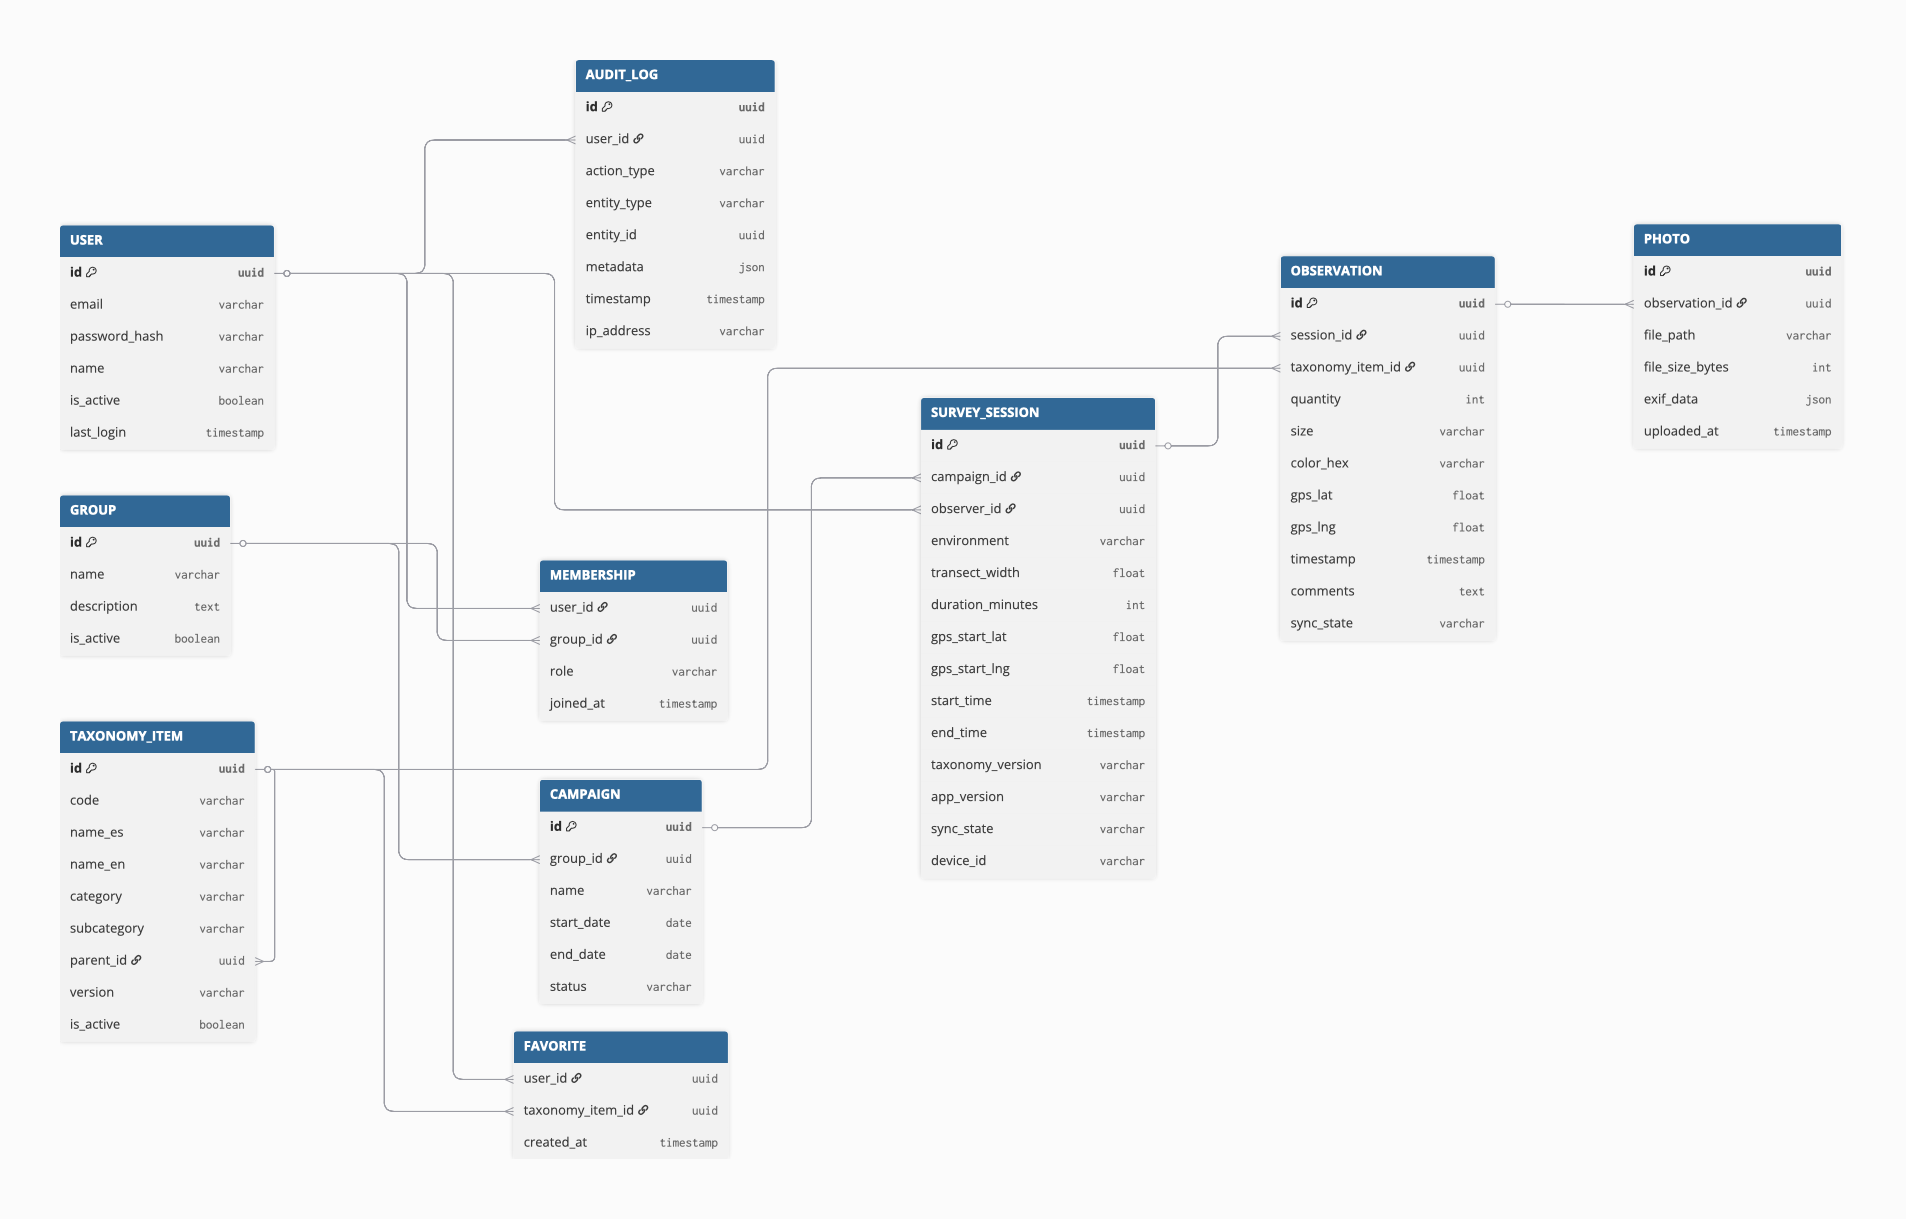
\includegraphics[width=\textwidth]{figures/modelo_er.png}
  \caption{Diagrama entidad-relación del sistema OmniLitter.}
  \label{fig:modelo_er}
\end{figure}


\subsubsection{Descripción de entidades}

La tabla~\ref{tab:entidades} describe los atributos clave de cada entidad y su
propósito en el sistema.

\begin{longtable}{p{3.2cm} p{4.2cm} p{6.6cm}}
  \caption{Descripción de entidades del modelo de datos.}
  \label{tab:entidades} \\
  \toprule
  \textbf{Entidad} & \textbf{Atributos principales} & \textbf{Descripción} \\
  \midrule
  \endfirsthead
  \toprule
  \textbf{Entidad} & \textbf{Atributos principales} & \textbf{Descripción} \\
  \midrule
  \endhead
  \bottomrule
  \endfoot

  \texttt{USER} &
    \texttt{id (UUID)}, \texttt{email}, \texttt{password\_hash}, \texttt{name},
    \texttt{is\_active}, \texttt{last\_login} &
    Representa a cada persona registrada en el sistema. Las contraseñas se almacenan
    como \textit{hash} bcrypt y nunca en texto plano. \\[4pt]

  \texttt{GROUP} &
    \texttt{id (UUID)}, \texttt{name}, \texttt{description}, \texttt{is\_active} &
    Equipo de investigación. Un grupo puede ser archivado sin eliminar sus datos
    históricos, preservando la trazabilidad científica. \\[4pt]

  \texttt{MEMBERSHIP} &
    \texttt{user\_id (FK)}, \texttt{group\_id (FK)},
    \texttt{role (admin|editor|viewer)}, \texttt{joined\_at} &
    Tabla de unión que asocia usuarios con grupos asignándoles un rol. Un mismo usuario
    puede tener roles distintos en grupos distintos. \\[4pt]

  \texttt{CAMPAIGN} &
    \texttt{id (UUID)}, \texttt{group\_id (FK)}, \texttt{name},
    \texttt{start\_date}, \texttt{end\_date}, \texttt{status} &
    Proyecto científico de muestreo. Agrupa varias sesiones de campo bajo un
    objetivo común (p.ej., «Monitoreo anual Playa de la Caleta 2026»). \\[4pt]

  \texttt{SURVEY\_SESSION} &
    \texttt{id (UUID)}, \texttt{campaign\_id (FK)}, \texttt{observer\_id (FK)},
    \texttt{environment}, \texttt{transect\_width}, \texttt{duration\_minutes},
    \texttt{gps\_start\_lat/lng}, \texttt{start\_time}, \texttt{end\_time},
    \texttt{taxonomy\_version}, \texttt{app\_version}, \texttt{sync\_state},
    \texttt{device\_id} &
    Sesión de muestreo individual en campo. Registra todos los metadatos científicos
    necesarios para la reproducibilidad: protocolo, versión de taxonomía utilizada y
    versión de la aplicación. El campo \texttt{sync\_state} gestiona el ciclo de vida
    de la sincronización. \\[4pt]

  \texttt{OBSERVATION} &
    \texttt{id (UUID)}, \texttt{session\_id (FK)},
    \texttt{taxonomy\_item\_id (FK)}, \texttt{quantity}, \texttt{size},
    \texttt{color\_hex}, \texttt{gps\_lat/lng}, \texttt{timestamp},
    \texttt{comments}, \texttt{sync\_state} &
    Registro de un ítem de residuo observado. Constituye la unidad mínima de dato
    científico del sistema. \\[4pt]

  \texttt{PHOTO} &
    \texttt{id (UUID)}, \texttt{observation\_id (FK)}, \texttt{file\_path},
    \texttt{file\_size\_bytes}, \texttt{exif\_data (JSONB)}, \texttt{uploaded\_at} &
    Imagen asociada a una observación. Los metadatos EXIF (coordenadas GPS
    embebidas en la imagen, fecha de captura, modelo de cámara) se almacenan en
    formato JSONB para máxima flexibilidad. \\[4pt]

  \texttt{TAXONOMY\_ITEM} &
    \texttt{id (UUID)}, \texttt{code}, \texttt{name\_es}, \texttt{name\_en},
    \texttt{category}, \texttt{subcategory}, \texttt{parent\_id (FK self-ref)},
    \texttt{version}, \texttt{is\_active} &
    Catálogo de tipos de residuo basado en la \textit{Joint List of Litter Categories}.
    La estructura jerárquica autorreferenciada (categoría → subcategoría → ítem)
    permite navegar la taxonomía sin conexión, ya que se descarga completa
    al iniciar sesión. \\[4pt]

  \texttt{FAVORITE} &
    \texttt{user\_id (FK)}, \texttt{taxonomy\_item\_id (FK)}, \texttt{created\_at} &
    Ítems de taxonomía marcados como favoritos por el usuario para agilizar la
    captura de observaciones en campo. \\[4pt]

  \texttt{AUDIT\_LOG} &
    \texttt{id}, \texttt{user\_id (FK)}, \texttt{action\_type},
    \texttt{entity\_type}, \texttt{entity\_id}, \texttt{metadata (JSONB)},
    \texttt{timestamp}, \texttt{ip\_address} &
    Registro de auditoría que almacena las acciones relevantes sobre el sistema
    (inicio de sesión, creación y edición de observaciones, exportaciones de datos,
    cambios de configuración). Garantiza la trazabilidad exigida en entornos de
    investigación científica. \\

\end{longtable}

\subsubsection{Decisiones de diseño de la base de datos}

\textbf{UUID como clave primaria universal.}
Todos los identificadores primarios son UUID v4 generados en el cliente (ya sea el
navegador o el dispositivo móvil). Esto resuelve el problema de colisiones de claves
en escenarios de creación offline: dos dispositivos diferentes que creen una observación
sin conexión obtendrán identificadores globalmente únicos que no entrarán en conflicto
cuando se sincronicen con el servidor.

\textbf{Rol en \texttt{MEMBERSHIP}, no en \texttt{USER}.}
El rol de un investigador no es una propiedad intrínseca de la persona, sino de su
relación con un grupo concreto. Un mismo investigador puede ser administrador en su
grupo principal y colaborador invitado en otro grupo. Modelar el rol en la tabla de
unión es, por tanto, la decisión correcta desde el punto de vista semántico.

\textbf{Versión de taxonomía en cada sesión y observación.}
La taxonomía de residuos evoluciona con el tiempo a medida que la comunidad científica
añade o reorganiza categorías. Registrar la versión exacta utilizada en cada sesión
permite reconstruir con exactitud qué definición se aplicó a cada observación, lo que
es un requisito básico de reproducibilidad científica.

\textbf{JSONB para metadatos heterogéneos.}
Los campos \texttt{exif\_data} y \texttt{metadata} utilizan el tipo JSONB de PostgreSQL
para almacenar datos cuya estructura puede variar (distintos modelos de cámara incluyen
campos EXIF diferentes, distintas acciones de auditoría tienen distintos contextos).
Esta decisión evita la proliferación de columnas opcionales con valor nulo y preserva
la flexibilidad para añadir nuevos atributos sin migrar el esquema.

% ------------------------------------------------------------
\subsection{Diseño de la API REST}
% ------------------------------------------------------------

La API sigue los principios REST: interfaz uniforme, comunicación sin estado,
recursos identificados por URI y representaciones en formato JSON. Todos los
\textit{endpoints} protegidos requieren el encabezado
\texttt{Authorization: Bearer <token>}, donde el \textit{token} es un JWT firmado
emitido en el \textit{endpoint} de autenticación.

La tabla~\ref{tab:endpoints} recoge los \textit{endpoints} principales agrupados
por recurso.

\begin{longtable}{p{1.5cm} p{5.5cm} p{2cm} p{4cm}}
  \caption{Principales \textit{endpoints} de la API REST de OmniLitter.}
  \label{tab:endpoints} \\
  \toprule
  \textbf{Método} & \textbf{Ruta} & \textbf{Protegido} & \textbf{Descripción} \\
  \midrule
  \endfirsthead
  \toprule
  \textbf{Método} & \textbf{Ruta} & \textbf{Protegido} & \textbf{Descripción} \\
  \midrule
  \endhead
  \bottomrule
  \endfoot

  \multicolumn{4}{l}{\textit{Autenticación}} \\[2pt]
  POST & \texttt{/api/auth/login} & No & Emite JWT de acceso y refresco \\
  POST & \texttt{/api/auth/refresh} & No & Renueva el JWT de acceso \\
  POST & \texttt{/api/auth/logout} & Sí & Invalida el \textit{token} de refresco \\[6pt]

  \multicolumn{4}{l}{\textit{Usuarios}} \\[2pt]
  GET  & \texttt{/api/users} & Sí (admin) & Lista todos los usuarios \\
  POST & \texttt{/api/users} & Sí (admin) & Crea un nuevo usuario \\
  GET  & \texttt{/api/users/:id} & Sí & Obtiene un usuario \\
  PATCH & \texttt{/api/users/:id} & Sí (admin) & Actualiza datos o estado \\[6pt]

  \multicolumn{4}{l}{\textit{Grupos}} \\[2pt]
  GET  & \texttt{/api/groups} & Sí & Lista grupos del usuario autenticado \\
  POST & \texttt{/api/groups} & Sí (admin) & Crea un grupo \\
  PATCH & \texttt{/api/groups/:id} & Sí (admin) & Edita nombre/descripción \\
  DELETE & \texttt{/api/groups/:id/archive} & Sí (admin) & Archiva un grupo \\
  POST & \texttt{/api/groups/:id/members} & Sí (admin) & Añade miembro \\
  DELETE & \texttt{/api/groups/:id/members/:uid} & Sí (admin) & Elimina miembro \\[6pt]

  \multicolumn{4}{l}{\textit{Sesiones de muestreo}} \\[2pt]
  GET  & \texttt{/api/sessions} & Sí & Lista sesiones accesibles \\
  POST & \texttt{/api/sessions} & Sí & Crea una sesión \\
  GET  & \texttt{/api/sessions/:id} & Sí & Obtiene una sesión con observaciones \\
  PATCH & \texttt{/api/sessions/:id} & Sí & Actualiza metadatos \\[6pt]

  \multicolumn{4}{l}{\textit{Observaciones}} \\[2pt]
  GET  & \texttt{/api/sessions/:id/observations} & Sí & Lista observaciones de sesión \\
  POST & \texttt{/api/sessions/:id/observations} & Sí & Registra una observación \\
  GET  & \texttt{/api/observations} & Sí & Lista todas (filtros opcionales) \\[6pt]

  \multicolumn{4}{l}{\textit{Fotos}} \\[2pt]
  POST & \texttt{/api/observations/:id/photos} & Sí & Sube una foto (multipart) \\
  GET  & \texttt{/api/photos/:id} & Sí & Sirve el archivo de imagen \\[6pt]

  \multicolumn{4}{l}{\textit{Taxonomía}} \\[2pt]
  GET  & \texttt{/api/taxonomy} & Sí & Descarga la taxonomía completa \\
  GET  & \texttt{/api/taxonomy?version=:v} & Sí & Descarga versión específica \\[6pt]

  \multicolumn{4}{l}{\textit{Sincronización}} \\[2pt]
  POST & \texttt{/api/sync/batch} & Sí & Sube cola de registros pendientes \\
  GET  & \texttt{/api/sync/changes} & Sí & Descarga cambios desde \texttt{last\_sync} \\[6pt]

  \multicolumn{4}{l}{\textit{Exportación}} \\[2pt]
  GET  & \texttt{/api/export/csv} & Sí (admin) & Exporta observaciones en CSV científico \\

\end{longtable}

\subsubsection{Autenticación y autorización}

El sistema implementa autenticación basada en JWT con dos \textit{tokens}: un
\textbf{token de acceso} de corta duración (15 minutos) y un \textbf{token de refresco}
de larga duración (7 días). El token de acceso se envía en cada petición en el encabezado
\texttt{Authorization}; el de refresco se utiliza exclusivamente para solicitar un nuevo
token de acceso cuando el anterior expira.

La autorización sigue un modelo de control de acceso basado en roles (RBAC)
a nivel de grupo. El \textit{middleware} de autorización verifica, para cada petición,
que el usuario autenticado posee el rol requerido en el grupo al que pertenece el
recurso solicitado. Esto permite que una misma persona sea administradora en un grupo
y colaboradora en otro, con permisos diferentes en cada contexto.

% ------------------------------------------------------------
\subsection{Diseño del Portal Web}
% ------------------------------------------------------------

\subsubsection{Arquitectura de componentes}

El portal web está implementado como una \textit{Single Page Application} (SPA) con
React 18 y TypeScript, empaquetada con Vite y estilizada con Tailwind CSS. La
navegación entre páginas es gestionada por React Router, que define dos niveles de rutas:

\begin{itemize}
  \item \textbf{Rutas públicas:} la página de inicio (\texttt{/}) y el formulario
    de inicio de sesión (\texttt{/login}), accesibles sin autenticación.
  \item \textbf{Rutas protegidas:} todas las páginas bajo \texttt{/app/*}, protegidas
    por un componente \texttt{PrivateRoute} que verifica el estado de autenticación y
    redirige al \textit{login} si no existe sesión activa.
\end{itemize}

La estructura de componentes sigue una jerarquía de tres niveles: el \texttt{Layout}
general (barra lateral, encabezado, selector de grupo activo) envuelve las páginas
individuales, que a su vez utilizan componentes reutilizables (tarjetas de estadística,
tablas filtrables, modales de confirmación).

\subsubsection{Gestión de estado}

El portal web utiliza \texttt{localStorage} como mecanismo de persistencia de la
sesión del usuario entre recargas de página, almacenando el JWT de acceso, el nombre
del usuario, su rol y el grupo activo seleccionado. Este enfoque es suficiente para
una SPA sin estado de servidor, y se complementará con manejo de \textit{refresh
token} en la implementación real.

La comunicación entre el selector de grupo activo (ubicado en la barra lateral) y el
componente Dashboard se implementa mediante un evento personalizado del DOM
(\texttt{omnilitter:groupChanged}), lo que evita prop-drilling innecesario sin
requerir una solución de gestión de estado global.

\subsubsection{Flujo de navegación y control de acceso por rol}

Las secciones de \textbf{Grupos} y \textbf{Usuarios} son exclusivas del rol de
administrador y no aparecen en la barra de navegación para los colaboradores.
El Dashboard ajusta el contenido mostrado según el rol: los administradores ven
estadísticas globales del grupo activo, mientras que los colaboradores ven únicamente
sus propias métricas. La tabla de observaciones filtra los registros por autor para los
colaboradores y muestra todos para los administradores.

% ------------------------------------------------------------
\subsection{Diseño de la Aplicación Móvil}
% ------------------------------------------------------------

\subsubsection{Stack tecnológico y estructura de pantallas}

La aplicación móvil está construida con \textbf{React Native} y \textbf{Expo bare
workflow}. La elección del \textit{bare workflow} frente al \textit{managed workflow}
responde a la necesidad de acceso completo a las APIs nativas del dispositivo: GPS
continuo con expo-location, captura de imagen con metadatos EXIF con expo-camera,
y sincronización en segundo plano con expo-background-fetch.

La navegación está organizada en dos niveles:

\begin{itemize}
  \item \textbf{Navegación de primer nivel (tab bar):} cinco pestañas inferiores
    (Inicio, Sesiones, Mapa, Sincronización, Perfil), visibles únicamente en las
    pantallas principales.
  \item \textbf{Navegación de pila (\textit{stack}):} flujos de varios pasos como la
    creación de una nueva sesión o la captura de una observación, que se presentan
    sin el \textit{tab bar}.
\end{itemize}

\subsubsection{Gestión de estado global}

El estado global de la aplicación se gestiona mediante el patrón
\textbf{Context + useReducer} de React, sin dependencias externas de gestión de
estado. El contexto \texttt{AppContext} expone el estado completo (sesiones activas,
tipos de residuo, datos del usuario, estado de sincronización) y un \textit{dispatcher}
con acciones tipadas en TypeScript. Este patrón proporciona la predictibilidad de
Redux con una superficie de código significativamente menor, adecuada para la escala
del proyecto.

\subsubsection{Base de datos local con WatermelonDB}

WatermelonDB actúa como base de datos local sobre SQLite. Se elige frente a SQLite
directo por tres razones: (1) está diseñado explícitamente para el patrón
\textit{offline-first} con sincronización en diferido; (2) ofrece un sistema de
consultas reactivo basado en observables que actualiza la UI automáticamente cuando
cambian los datos; (3) su rendimiento en colecciones grandes (miles de observaciones)
es significativamente superior al de SQLite gestionado manualmente.

El esquema local replica el subconjunto del modelo de datos necesario para la
operación en campo: \texttt{survey\_sessions}, \texttt{observations}, \texttt{photos}
y \texttt{sync\_queue}, además de la taxonomía completa cargada al iniciar sesión.

\subsubsection{Flujo de captura de una observación}

El flujo principal de la aplicación sigue esta secuencia:

\begin{enumerate}
  \item El investigador inicia una nueva sesión de muestreo, especificando el nombre,
    el tipo de entorno y los parámetros del transecto.
  \item Para cada ítem encontrado, abre la pantalla de nueva observación, selecciona
    el tipo de residuo a través del modal de taxonomía (organizado en cuadrícula visual
    por categorías e iconos), e introduce cantidad, tamaño, color y comentarios.
  \item Opcionalmente captura una foto geolocalizada del residuo.
  \item Al finalizar la sesión de campo, revisa el resumen y puede iniciar la
    sincronización manualmente o dejar que se realice en segundo plano al recuperar
    cobertura de red.
\end{enumerate}

% ------------------------------------------------------------
\subsection{Mecanismo de Sincronización Offline}
% ------------------------------------------------------------

\subsubsection{Patrón Outbox Queue}

El mecanismo de sincronización implementa el patrón \textbf{Outbox Queue}
(cola de salida), ampliamente utilizado en sistemas distribuidos con conectividad
intermitente. El funcionamiento es el siguiente:

\begin{enumerate}
  \item Cuando el usuario crea o modifica un registro (sesión u observación) en el
    dispositivo sin conexión, el registro se persiste en WatermelonDB con
    \texttt{sync\_state = PENDING} y se inserta una entrada en la tabla
    \texttt{sync\_queue} con el \textit{payload} completo del cambio.
  \item Cuando el dispositivo recupera conectividad, \texttt{expo-background-fetch}
    activa el proceso de sincronización, que lee la cola y realiza una petición
    \texttt{POST /api/sync/batch} con todos los registros pendientes.
  \item El servidor procesa los registros en orden, los persiste en PostgreSQL y
    devuelve el estado canónico actualizado.
  \item El cliente actualiza el \texttt{sync\_state} de los registros procesados a
    \texttt{SYNCED} y descarga los cambios remotos realizados por otros usuarios
    mediante \texttt{GET /api/sync/changes?since=\{last\_sync\_timestamp\}}.
  \item En caso de error en un registro concreto (conflicto de datos, registro
    inválido), ese registro pasa a \texttt{sync\_state = ERROR} y se notifica al
    usuario, sin bloquear la sincronización del resto.
\end{enumerate}

\subsubsection{Estados de sincronización}

Cada sesión y observación puede encontrarse en uno de cuatro estados, como muestra
la tabla~\ref{tab:sync_states}.

\begin{table}[H]
  \centering
  \caption{Estados de sincronización y su significado.}
  \label{tab:sync_states}
  \begin{tabularx}{\textwidth}{lX}
    \toprule
    \textbf{Estado} & \textbf{Significado} \\
    \midrule
    \texttt{PENDING}  & El registro existe solo en el dispositivo; aún no se ha
                        intentado sincronizar. \\
    \texttt{SYNCING}  & El registro está siendo procesado en la petición de
                        sincronización actual. \\
    \texttt{SYNCED}   & El servidor ha confirmado la recepción y persistencia del
                        registro. \\
    \texttt{ERROR}    & El servidor rechazó el registro (conflicto, datos inválidos).
                        Requiere intervención manual o reintento. \\
    \bottomrule
  \end{tabularx}
\end{table}

\subsubsection{Resolución de conflictos}

La estrategia de resolución de conflictos adoptada es \textbf{last-write-wins} con
granularidad de registro: si dos usuarios modifican la misma sesión de forma
independiente mientras están sin conexión, prevalece la versión con el
\texttt{timestamp} más reciente. Esta estrategia es suficiente para el modelo de uso
de OmniLitter, donde cada sesión de muestreo pertenece a un único observador
responsable y los conflictos genuinos son infrecuentes.

\subsubsection{Garantía de identificadores únicos en entorno offline}

Para que la estrategia Outbox Queue funcione sin servidor central asignando IDs,
todos los identificadores del sistema son \textbf{UUID v4 generados en el cliente}.
Esto garantiza que los registros creados simultáneamente en distintos dispositivos
nunca colisionarán al sincronizarse, independientemente del orden de llegada al
servidor.
